\documentclass[12pt]{article}
\usepackage[margin=2.5cm]{geometry}
\usepackage{enumerate}
\usepackage{amsfonts}
\usepackage{amsmath}
\usepackage{fancyhdr}
\usepackage{amsmath}
\usepackage{amssymb}
\usepackage{amsthm}
\usepackage{mdframed}
\usepackage{graphicx}
\usepackage{subcaption}
\usepackage{adjustbox}
\usepackage{listings}
\usepackage{xcolor}
\usepackage{booktabs}
\usepackage[utf]{kotex}
\usepackage{hyperref}

\definecolor{codegreen}{rgb}{0,0.6,0}
\definecolor{codegray}{rgb}{0.5,0.5,0.5}
\definecolor{codepurple}{rgb}{0.58,0,0.82}
\definecolor{backcolour}{rgb}{0.95,0.95,0.92}

\lstdefinestyle{mystyle}{
    backgroundcolor=\color{backcolour},
    commentstyle=\color{codegreen},
    keywordstyle=\color{magenta},
    numberstyle=\tiny\color{codegray},
    stringstyle=\color{codepurple},
    basicstyle=\ttfamily\footnotesize,
    breakatwhitespace=false,
    breaklines=true,
    captionpos=b,
    keepspaces=true,
    numbers=left,
    numbersep=5pt,
    showspaces=false,
    showstringspaces=false,
    showtabs=false,
    tabsize=1
}

\lstset{style=mystyle}

\pagestyle{fancy}
\renewcommand{\headrulewidth}{0.4pt}
\lhead{Team Treehouse}
\rhead{Reporting with SQL Part 3 Notes}

\begin{document}
\title{Reporting with SQL Part 3 Notes}
\author{Team Treehouse}
\maketitle

\bigskip

\section{Counting Results}

\bigskip

\begin{itemize}
    \item \textbf{Syntax 1:} SELECT COUNT(\textit{column name}) FROM \textit{table name};
    \begin{itemize}
        \item Counts all non-null values
    \end{itemize}
    \item \textbf{Syntax 2:} SELECT COUNT(*) FROM \textit{table name};
    \begin{itemize}
        \item counts all rows in a table
    \end{itemize}
    \item \textbf{Syntax 2:} SELECT COUNT(DISTINCT \textit{column name}) FROM \textit{table};
    \begin{itemize}
        \item Counts all items with distinct value in a column
    \end{itemize}

    \bigskip

    \underline{\textbf{Example:}}

    \bigskip

    \begin{lstlisting}[language=SQL]
    SELECT COUNT(DISTINCT category) FROM products;


    SELECT COUNT(*) FROM customers ORDER BY id DESC LIMIT 1;
    \end{lstlisting}

\end{itemize}

\bigskip

\section{Exercise 1}

\bigskip

\begin{itemize}
    \item Solution included in \textit{exercise\_1.sql}
\end{itemize}

\bigskip

\section{Counting Groups of Rows}

\bigskip

\begin{itemize}
    \item \textbf{Syntax:} SELECT COUNT(\textit{column name}) FROM \textit{table name} GROUP BY \textit{column name with common value};
    \item is almost like using keyword distinct
    \begin{itemize}
        \item SELECT COUNT(DISTINCT \textit{column name}) FROM \textit{table};
    \end{itemize}
    \item but, group by allows to add additional columns

    \bigskip

    \underline{\textbf{Exxample:}}

    \bigskip

    \begin{lstlisting}[language=SQL]
    SELECT category, COUNT(*) AS product_count FROM products GROUP BY category;
    \end{lstlisting}

    \bigskip

    \begin{center}
    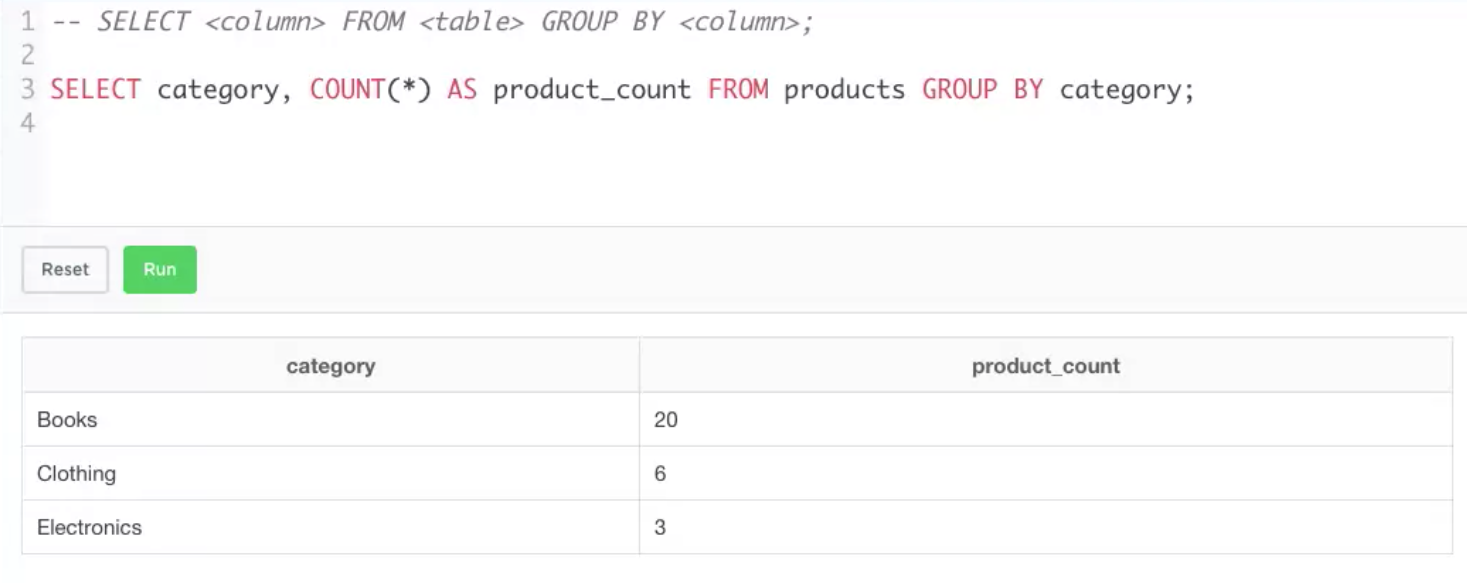
\includegraphics[width=\linewidth]{images/part_3_notes_1.png}
    \end{center}
\end{itemize}

\bigskip

\section{Exercise 2}

\bigskip

\begin{itemize}
    \item Solution included in \textit{exercise\_2.sql}
\end{itemize}

\bigskip

\section{Getting the Grand Total}

\bigskip

\begin{itemize}
    \item SUM
    \begin{itemize}
        \item \textbf{Syntax:} SELECT SUM(\textit{numeric column}) FROM \textit{table name};

    \bigskip

    \underline{\textbf{Example:}}

    \bigskip

    \begin{lstlisting}[language=SQL]
    SELECT SUM(cost) AS total_spend, user_id FROM orders GROUP BY user_id;
    \end{lstlisting}

    \bigskip

    \begin{center}
    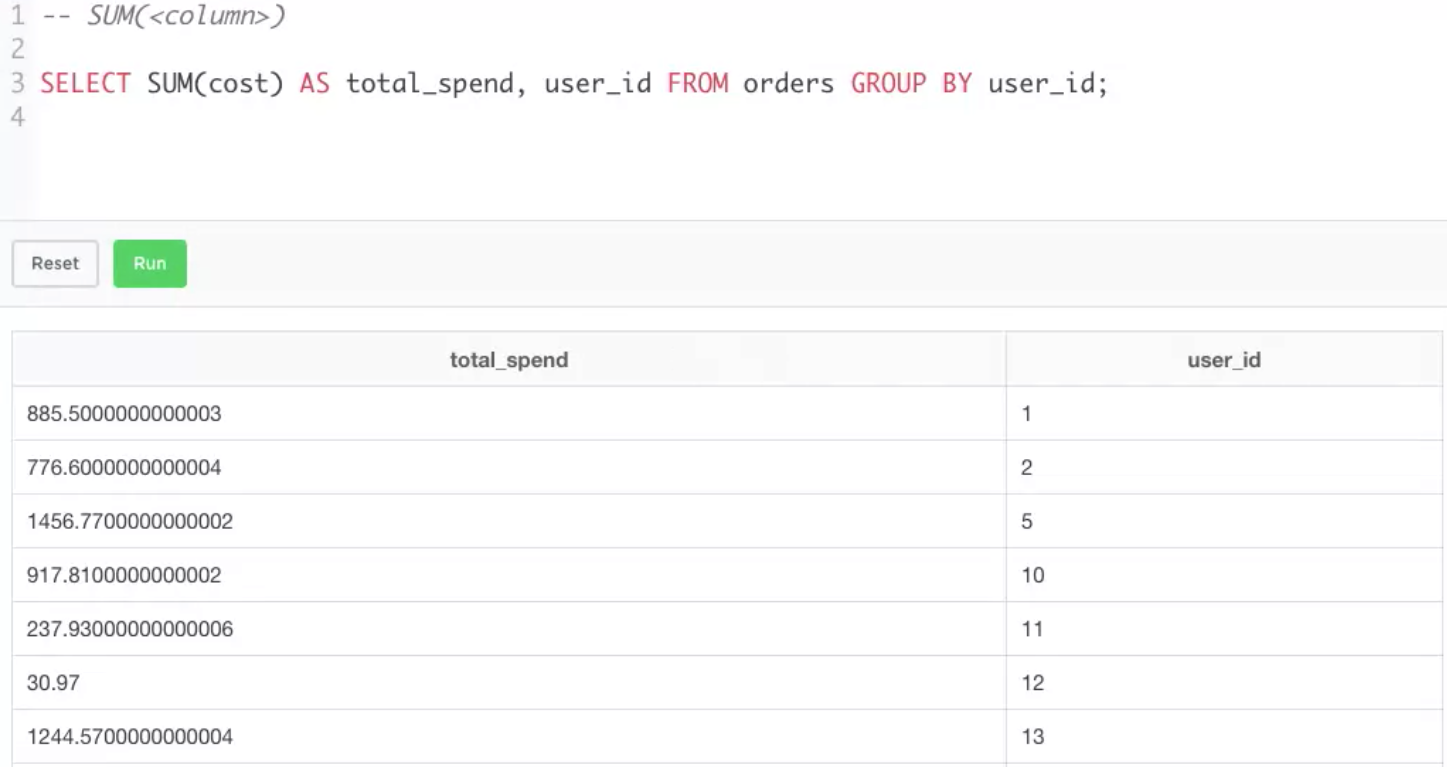
\includegraphics[width=\linewidth]{images/part_3_notes_2.png}
    \end{center}

    \end{itemize}
    \item SUM with GROUP BY and WHERE
    \begin{itemize}
        \item Not possible, but there is an alternative, HAVING
        \item \textbf{Syntax:} SELECT SUM(\textit{numeric column name}) AS \textit{alias} FROM \textit{table name}
        GROUP BY \textit{another column name} HAVING \textit{alias} \textit{operator} \textit{value};

        \bigskip

        \underline{\textbf{Example:}}

        \bigskip


    \begin{lstlisting}[language=SQL]
    SELECT SUM(cost) AS total_spend, user_id FROM orders
        GROUP BY user_id
        HAVING total_spend > 250
        ORDER BY total_spend DESC;
    \end{lstlisting}

        \bigskip

        \begin{center}
        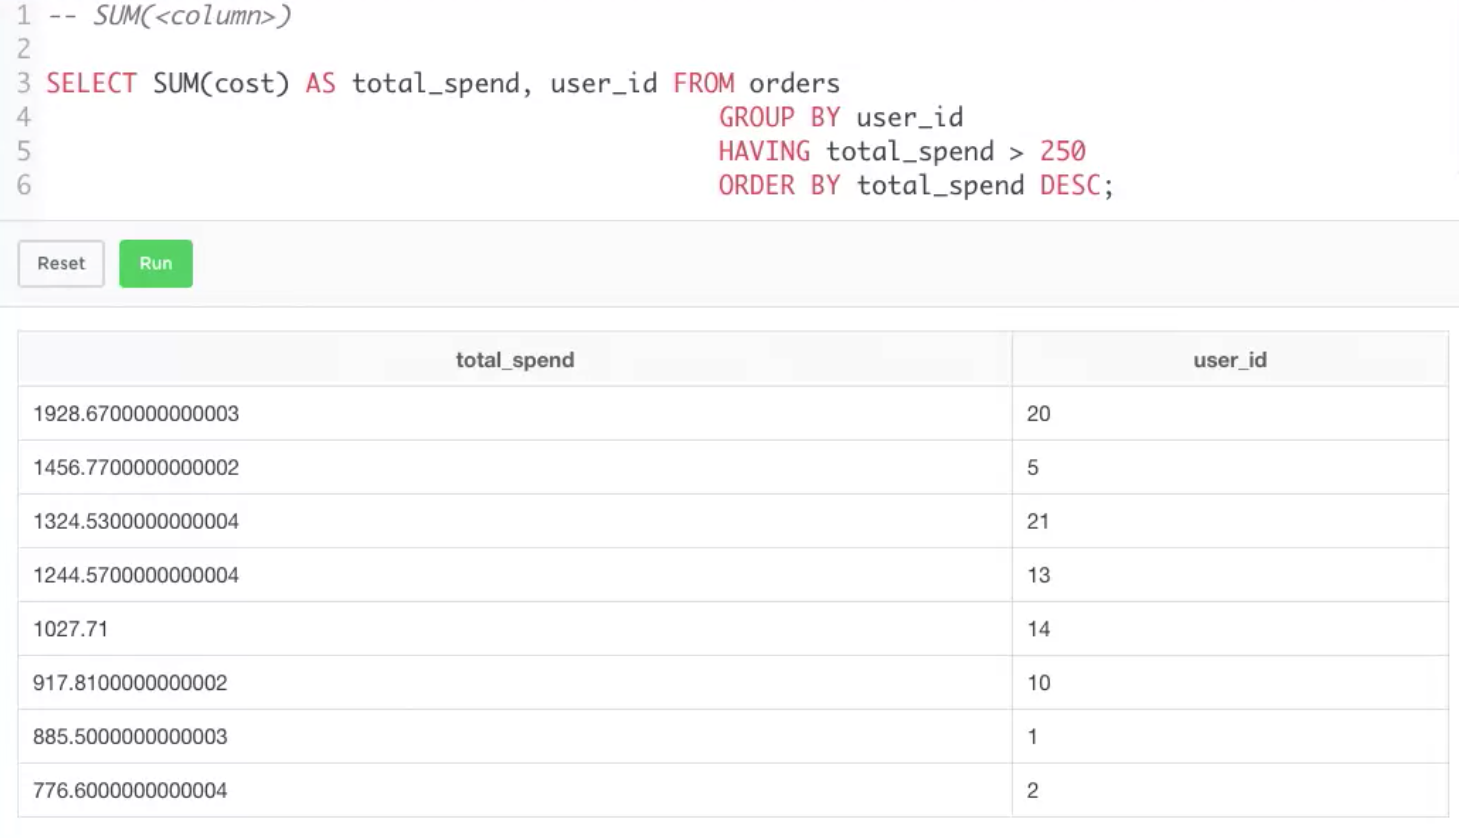
\includegraphics[width=\linewidth]{images/part_3_notes_3.png}
        \end{center}

    \end{itemize}
\end{itemize}

\end{document}